
%% CLASS MANUAL FOUND IN http://blog.poormansmath.net/latex-class-for-lecture-notes/ %%
%% CLASS AUTHOR Stefano Maggiolo %%
\documentclass[english,course]{Notes}

\title{Computer Systems 1}
\subject{Computer Systems}
\author{Joao Almeida-Domingues}
\email{2334590D@student.gla.ac.uk}
\speaker{Dr. John T. O'Donnell}
\date{07}{01}{2019}
\dateend{24}{05}{2019}
\place{University of Glasgow}

\usepackage[backend=biber, style=reading]{biblatex}
\bibliography{CSbiblio}

\graphicspath{{assets/}}

%%%%circuits
\usepackage{circuitikz, float}

 %%%%% GENERAL MATHEMATICAL NOTATION SHORTCUTS %%%%%
 
\newcommand{\n}{\mathbb{N}}
\newcommand{\z}{\mathbb{Z}}
\newcommand{\q}{\mathbb{Q}}
\newcommand{\cx}{\mathbb{C}}
\newcommand{\real}{\mathbb{R}}
\newcommand{\field}{\mathbb{F}}
\newcommand{\ita}[1]{\textit{#1}}
\newcommand{\oneton}{\{1,2,3,...,n\}}
\newcommand\ef{\ita{f} }
 %\qedhere to force QED in place
\newcommand\inv[1]{#1^{-1}}
\newcommand\setb[1]{\{#1\}}
\newcommand\en{\ita{n }}
\renewcommand\qedsymbol{QED} %QED instead of square


%%%%%%%%%%%%%%%%PACKAGES%%%%%%%%%%%%%%%%%%%%%%%%%%%%%
%\usepackage{lipsum}  

\usepackage{amsmath,amsthm,amssymb,graphicx,mathtools,tikz} %maths
\usepackage{hyperref,framed,color,fancybox} %layout


% framed :  \begin{shaded,frame,snugshade or leftbar} \definecolor{shadecolor}{rgb}{XYZ} to change color
%fancybox: \shadowbox,ovalbox or doublebox
%\extra for Extra content layout box
%%%%%%%%%%%%%%%%%%%%%%%%%%%

%%%CLASS SHORTCUTS%%%%
%\lecture{day}{month}{year} for margin note 
%\begin{theorem} sdfsdf\end{theorem}  --> \theorem
%\begin{proposition} dfsdfs\end{proposition} --> \prop
%\begin{lemma} dsfsd \end{lemma} --> \lem
%\begin{corollary} f ffew \end{corollary}
%\begin{definition} fwewef w \end{definition} --> \defn
%\begin{example} feww e\end{example} --> \ex
%\begin{exercise} wefwe \end{exercise}
%\begin{remark} wef we \end{remark} --> \rem
%\begin{fact} wefe \end{fact}
%\begin{problem} wef ew \end{problem}
%\begin{conjecture} ewfew \end{conjecture}
%\begin{claim} few w \end{claim}
%\begin{notation} fewf \end{notation} --> \nota
%\mymarginpar for scriptsize margin

\begin{document}
\newpage

\section{Analogue and Digital Representation}

\subsection{Computer Systems}

\lecture{08}{01}{2019}

\defn{Digital Circuits}{Electronic systems which use very large numbers of only a few types of components, which when connected the right way create incredibly complex , useful behaviour}

\defn{Machine Language}{Programming language executed directly by the computer hardware, which serves as the interface between low-level circuits and high-level software. Therefore, it is simple enough so that a digital circuit can be designed to execute it, yet also powerful enough that high-level languages can be converted into it}


\subsection{Data Representation}

\par{There are several digital data types which need somehow be represented in hardware. This is done by encoding electrical signals (voltage). It is by manipulating these voltages in the hardware that computations are able to be performed. There are 2 ways of achieving this:}

\begin{enumerate}
	\item \textbf{Analogue}
	
		\defn{}{The variables in the calculation are \ita{analogue} to the physical signals being measured (e.g. $1 \iff 3$v)}
		
		\par{There are some advantages to this method, such as fast calculation of differential equations. Unfortunately, it also has significant drawbacks: limited precision; errors accumulate; difficult to represent non-numerical data}
		
	\item \textbf{Digital}
	
		\defn{}{As indicated by the root of the word, it makes use of digits. It is by counting that calculations can be performed.}
		
		\par{This addresses some of the drawbacks of analogue computing. For example, one can always add more digits when higher precision is required; Handles noise and errors better; Easy representation of most data types}
		
\end{enumerate}

	\defn{Bit}{Unit of information used in digital circuits. It represents either a $0$ or a $1$}
	
	\rem{Different circuits use different voltages, but the more simpler and reliable ones tend to use just two clearly distinct voltages to represent each value $(0,1)$ }
	
	\defn{Flip Flop}{The simplest circuit with memory. Basic element of computer memory}
	
	\defn{Byte}{8 bits}
	
	\par{Note that just like in any other positional number system, the number of possible representations grows exponentially with the number of digits added. In the binary system we only have $0 , 1$. But by using basic knowledge of combinatorics, one observes that for every new position $n$ the number of possible orderings doubles. It follows, for example, that for an 8 bit binary number one can represent up to $2^8 = 256$ different values ( $0 \to 255$ ). In general, for a $k$ bit number:
	
	$$ 2^k \text{ possible values. From 0 until } 2^k - 1$$ 
	
	\nota{ By convention, 4 bits are separated by a space for readability $$0000 \ 0000$$}
	
	\defn{Word}{For convenience, for larger numbers of bits, the term \ita{word} is used. The specific number of bits which a word represent changes. For this class: $16, 32 , 64 = $ short w., w., long w.}
	
\lecture{10}{01}{2019}

	\section{Number Systems}
	
	\subsection{Conversion}
	
	\par{Conversions between different bases are easily achieved, by keeping in mind the simple fact that each position is able to represent a minimum value, and a maximum value, every time that value is exceeded , we need another "slot" to reset the counting with the "symbols" (i.e the digits) available in that system. To make it clear, let's first look at the decimal system, as first learned in primary school. $19_{10}$ can be thought of $10 + 9$ , which in turn can be thought of 9 single units + 1 single "10" unit. Since 9 is the highest "unit symbol" available in the decimal number system we need another slot "the tenths". Transitioning from $9$ to  "10". Note how the "counter" was reset to $0$ and we now start counting again from 1, but in the tenths and in the units slot. We don't need to add another slot until all digits, in all possible combinations have been used.}
	\par{Similarly, binary/base 2, simply means that for every "slot" we have only two "symbols" at our disposal, $0$ and $1$. And instead of thinking of the slots as $10^{ths} , 100^{ths} , \dots$ we think in terms of powers of $2$.}
	
	$$
	\begin{tabular}{|c|c|c|c|c|c|c|c|c|c|c} 
	 $128$  & $64$ & $32$ & $16$ & & $8$  & $4$ & $2$ & $1$ \\
	      $2^7$ & $2^6$ & $2^5$ & $2^4$  & & $2^3$ & $2^2$ & $2^1$ & $2^0$ \\
	     $0$&$0$&$0$&$0$& & $0$&$1$&$1$&$1$& $= 4 + 2 + 1 = 7_ {10}$ 
	 \end{tabular}$$
	 
	 \newpage
	 \par{From decimal to binary the process is similar, but in reverse. If a primary school child was given a decimal table, and was  asked to fill it with $150$ , she would obviously not start by the units and start incrementing 1-by-1. She would notice that she'll need at least the 1 unit of "100" ($10^3$) and immediately put a 1 in the 3rd slot, and then notice that she'll need 5 "10s" and so on. This is trivial, and similarly trivial it is for base 2. Say you're given $74_{10}$. What is the highest slot you can immediately fill? Well, $128$ it's too high, the one before it is $64 = 2^7$ (position 7). That works, but it still leaves us with $10$ units to be represented. Repeating the process, we see that we'll need an $8 = 2^3$ (position 3) and a $2$ (position 2) until all units have been distributed amongst the "slots". Giving us: }
	 $$0 1 0 0  \ 1 0 1 0$$
	 
	 	     \par{This process is less straightforward for other bases, simply because we're used to think in base10. But the method is similar for all. Another useful base is \textbf{base 16}, where we use the letters A - F to represent the numbers from $10 \to 15$. This has the obvious advantage of reducing the number of "symbols"/characters needed for representing a binary number. For example: an 8 bit number can be easily represented by just 2 characters, with plenty leftover, since $16^2 = 256$ possible values.}
		     \nota{For this class "\$" is used to represent hexadecimal numbers}
		     
		     \par{The simplest way to convert from Binary to Hex is simply to note that, we need 4 bits to represent 1 hexadecimal bit in its entirety (i.e. $0$ - F) . Hence we split the number into 4 bit chunks and convert them into the corresponding hex character. Such that the first 4 bits correspond to the hex uni bit , the next 4 bits to the "$16^{ths}$" , etc.}
		     
		   $$ \begin{tabular}{|c|c|c|c|c|c|c|c|c|c|}
		      $0$&$1$&$0$&$0$& & $1$&$0$&$1$&$0$ \\
		      \hline
		      \multicolumn{4}{c} 4 & & \multicolumn{4}{c} A 
		      \end{tabular}$$
		      
		      \par{The reverse is done in the same way as in the decimal above, but again working only in 4 bit chunks}
		      \rem{Note however that it is always more natural to filter through decimal instead of thinking "$2^4 - 1 =$ F"}		     
	     
	     \subsection{Operations}

	\par{Multiplication and Addition are performed much like in the same way we perform operations in decimal, again keeping in mind the digits available to work within each system, every time we exceed the limit we must carry onto the next.}
	
	\par{Subtraction can be seen as a special case of addition with negative numbers, i.e. $3 - 2 = 3 + (-2)$. Binary numbers cannot represent negative numbers however, so we use \textbf{2's complement}. A 2c number is negative if its leftmost digit is $1$}
	
	\newpage
	\rem{Note that this does not affect the number of possible values that can still be represented, but it reduces the possible positive number representations in half, since for every positive number there will be a corresponding negative.\mymarginpar{except from the lowest possible negative, which positive counterpart will always need an extra bit, since we're counting from 0}}
	
	\par{The general conversion method is straight forward:}
	\begin{enumerate}
		\item Invert the bits
		\item Add 1
	\end{enumerate}
	
	\par{It can be useful to think of the rightmost digit of an $n$ bit 2c number as always representing the sum of  the highest possible negative number ($-2^{(n-1)}$) with an $n-1$ bits positive number. The $n^{th}$ bit is just the sign bit }
	
	\rem{Note that, by adding all the positives we'll get $0$, in which case the sign bit is turned off. We can think of $0$ as belonging to the positives in this case, since it has the sign bit off. But when not considering it, even though we can represent $2^{(n-1)}$ negative numbers we can only represent $2^{(n-1)} - 1$. Since the "$n^{th}$" would in effect be $0$.}
	
	\ex{ \begin{tabular}{c|c|c|c|c}
		      $1$&$0$&$1$&$0$ \\
		      $-8$&$+0$&$+2$&$+0$&$ = -6$
		\end{tabular} \\
		
		\par{Since it is a $2c$ number we know we can represent up to $2^3 = 8$ different values in each "direction" (considering 0 a positive number). So we have $-8$ and then we need to find out the 3bit binary. ($0\cdot2^0 + 1\cdot2^1 + 0\cdot2^2 = 2$). And then add them}
		
		}
		
	\par{It is clear from the example above how subtraction and division can then be performed just like addition}

\newpage

\section{Logic Gates}

\lecture{15}{01}{2019}

\defn{Logic Gate}{A physical, basic component, which takes $1+$ input(s) and performs a boolean function (i.e the result is either T/F) }

\begin{enumerate}

	\item \textbf{Inverter}
	
	\defn{}{Takes an input and returns its opposite}
	
	\nota{inv}
	
	\begin{minipage}[c]{.5\textwidth}
	\begin{circuitikz} \draw
		(0,2) node[american not port] (inv1) {};
	\end{circuitikz}
	\end{minipage}
	\mymarginpar{*alternatively $\bar{p}$}
	\begin{minipage}[c]{.5\textwidth}
	\begin{tabular}{|c|c|}
		$p$ & $\neg  p^*$  \\
		\hline
		1 & 0 \\
		0 & 1
	\end{tabular}
	\end{minipage}
	
	\item \textbf{2-Input AND}
	
	\defn{}{Returns true \ita{iff} the two inputs are true}
	
	\nota{and2 \mymarginpar{the 2 used in the gates' names just means that 2 inputs are passed}}
	
	\begin{minipage}[c]{.5\textwidth}
	\begin{circuitikz} \draw
		(0,2) node[american and port] (and2) {};
	\end{circuitikz}
	\end{minipage}
	\begin{minipage}[c]{.5\textwidth}
	\begin{tabular}{|c|c|c|}
		$p$ & $q$ & $p \land q$  \\
		\hline
		1 & 0 & 0 \\
		1 & 1 & 1 \\
		0 & 0 & 0 \\
		0 & 1 & 0
	\end{tabular}
	\end{minipage}
	
	\rem{Note that for a $n$ input truth-table, there are $2^n$ possible input combos}
	\rem{An easy way to construct truth tables is to start half(1)-half($0$), then $\tfrac{1}{4}, \ \tfrac{1}{8} , \cdots$.  So for a 3 input table, one first put 4 1s, 4 $0$s. Then, half of that, i.e. 2 1s 2 $0$s 2$\times$, and finally 1, $0$ , 8$\times$}
	
	\item \textbf{2-input OR}
	\defn{}{Returns true if any one of the two inputs are true, or if both are true}
	
	\nota{or2}
	
	\begin{minipage}[c]{.5\textwidth}
	\begin{circuitikz} \draw
		(0,2) node[american or port] (or2) {};
	\end{circuitikz}
	\end{minipage}
	\begin{minipage}[c]{.5\textwidth}
	\begin{tabular}{|c|c|c|}
		$p$ & $q$ & $p \lor q$  \\
		\hline
		1 & 0 & 1 \\
		1 & 1 & 1 \\
		0 & 0 & 0 \\
		0 & 1 & 1
	\end{tabular}
	\end{minipage}
	
	\newpage
	\item \textbf{2-input XOR}
	
	\defn{}{Returns true \ita{iff} one of the two inputs is true}
	
	\nota{xor2} \mymarginpar{*$\oplus$}
	
	\begin{minipage}[c]{.5\textwidth}
	\begin{circuitikz} \draw
		(0,2) node[american xor port] (xor2) {};
	\end{circuitikz}
	\end{minipage}
	\begin{minipage}[c]{.5\textwidth} 
	\begin{tabular}{|c|c|c|}
		$p$ & $q$ & $p \ \underline{\lor}* \ q$  \\
		\hline
		1 & 0 & 1 \\
		1 & 1 & 0 \\
		0 & 0 & 0 \\
		0 & 1 & 1
	\end{tabular}
	\end{minipage}
	
	\end{enumerate}
	

\subsection{Combinational Circuits}
	
\defn{Combinational Circuits}{Their output depends only on their current input. There's no feedback loop, or "memory" state}

\par{For complex circuits it is hard to keep track of every input and output by just connecting single logic gates. It is useful to create \ita{black box circuits} to abstract some of the complexity out. These components, regardless of what logic gates are used to built them*\mymarginpar{*hence the name black box}, always perform the same operation (e.g. choosing between two inputs).}

\begin{enumerate}

	\item \textbf{Multiplexer}
	
	\nota{mux1}
	
	\defn{}{Hardware equivalent of the \ita{"if-then-else"} statement. Chooses between 2 values ($x,y$) given a third ($c$). If $c$ $y$, else $x$}
	
	\rem{Every decision a computer makes comes down to a multiplexer}
	
	\begin{minipage}{\linewidth}
      \centering
      \begin{minipage}{0.45\linewidth}
          \begin{figure}[H]
              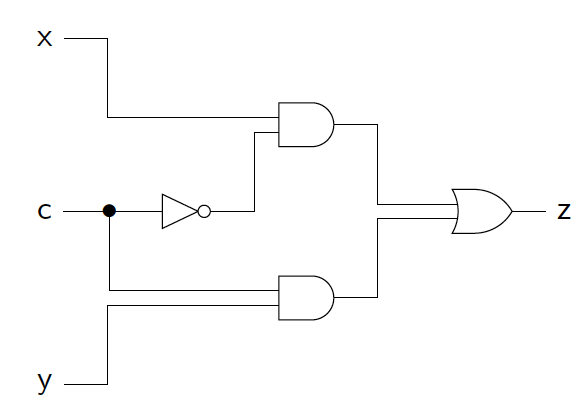
\includegraphics[width=\linewidth]{mux.png}
          \end{figure}
      \end{minipage}
      \hspace{0.05\linewidth}
      \begin{minipage}{0.45\linewidth}
      \begin{tabular}{|c|c|c|c|}
		$c$ & $x$ & $y$ & $z$  \\
		\hline
		$1$ & $1$ & $1$ & $1$ \\
		$1$ & $1$ & $0$ & $0$ \\
		$1$ & $0$ & $1$ & $1$ \\
		$1$ & $0$ & $0$ & $0$ \\ 
		$0$ & $1$ & $1$ & $1$ \\ 
		$0$ & $1$ & $0$ & $1$ \\
		$0$ & $0$ & $1$ & $0$ \\ 
		$0$ & $0$ & $0$ & $0$ \\
	\end{tabular}
	\end{minipage}
\end{minipage}
	
\newpage
	\item \textbf{Half-Adder}
	
	\defn{}{Adds two bits using a 2-bit (carry,sum) representation.}
	
	\par{Note that there's only a carry if both inputs are 1, hence we represent this by an and2 gate, while the sum can be represented by an xor2}
	
	\begin{minipage}{\linewidth}
      \centering
      \begin{minipage}{0.45\linewidth}
          \begin{figure}[H]
              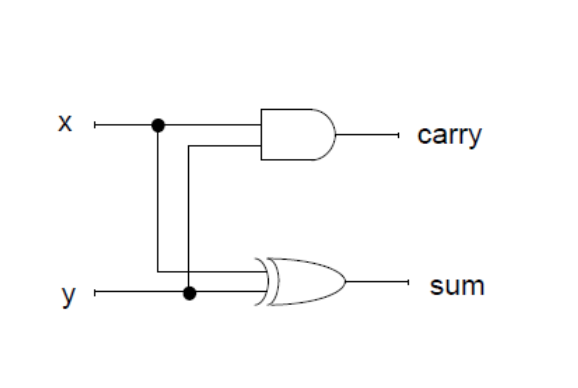
\includegraphics[width=\linewidth]{halfAdder.png}
          \end{figure}
      \end{minipage}
      \hspace{0.05\linewidth}
      \begin{minipage}{0.45\linewidth}
      \begin{tabular}{|c|c|c|c|}
		$x$ & $y$ & $c (x \land y)$ & $s (x \ \underline{\lor}  \ y)$  \\
		\hline
		$1$ & $1$ & $1$ & $0$ \\
		$1$ & $0$ & $0$ & $1$ \\
		$0$ & $1$ & $1$ & $1$ \\
		$0$ & $0$ & $0$ & $0$ \\ 
	\end{tabular}
	\end{minipage}
	
\end{minipage}

\item \textbf{Full-Adder}
	
	\defn{}{Adds three bits (inputs + carry) using a 2-bit (carry,sum) representation.}
	
	\par{Note that there's only a carry when 2+ inputs are 1, and there's only a sum iff there are an odd number of inputs equal to 1}
	
	\begin{minipage}{\linewidth}
      \centering
      \begin{minipage}{0.65\linewidth}
          \begin{figure}[H]
              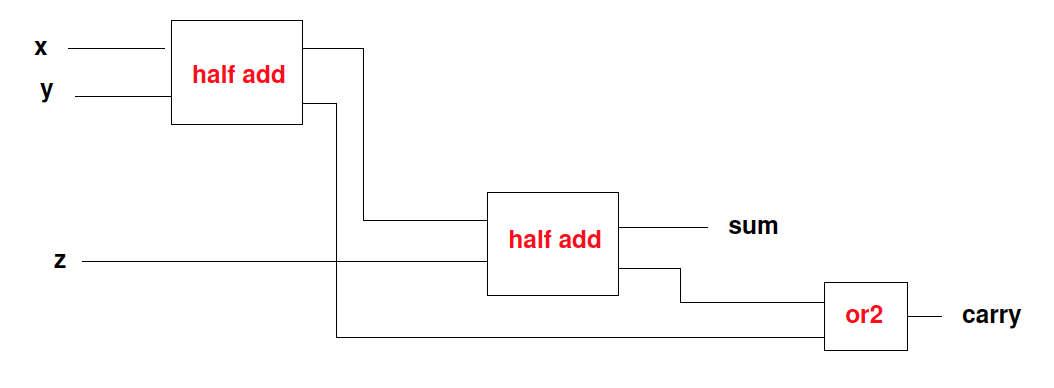
\includegraphics[width=\linewidth]{fullAdder.png}
          \end{figure}
      \end{minipage}
      \hspace{0.05\linewidth}
      \begin{minipage}{0.25\linewidth}
      \begin{tabular}{|c|c|c|c|c|}
		$x$ & $y$ & $z$ & $c$ & $s$  \\
		\hline
		$1$ & $1$ & $1$ &  $1$ & $1$ \\
		$1$ & $1$ & $0$ &  $1$ & $0$ \\
		$1$ & $0$ & $1$ &  $1$ & $0$ \\
		$1$ & $0$ & $0$ &  $0$ & $1$ \\ 
		$0$ & $1$ & $1$ &  $1$ & $0$ \\ 
		$0$ & $1$ & $0$ &  $0$ & $1$ \\
		$0$ & $0$ & $1$ &  $0$ & $1$ \\ 
		$0$ & $0$ & $0$ &  $0$ & $0$ \\
	\end{tabular}
	\end{minipage}
	
\end{minipage}
\end{enumerate}

\newpage
\section{Boolean Algebra \& Arithmetics}
\lecture{17}{01}{2019}
\subsection{Laws}

\defn{Idempotence}{operation that can be applied several times without changing the result}

$$ x \lor x = x \quad \quad x \land x = x$$

\defn{Commutative}{operations can be performed in any order}

$$ x \lor y = y \lor x \quad \quad x \land y = y \land x $$

\defn{Associative}{the order in which the operations are performed does not matter as long as the sequence of the operands is not changed}

$$\begin{array} { l } { x \lor ( y \lor z ) = ( x \lor y ) \lor z } \\ { x \land ( y \land z ) = ( x \land y ) \land z } \end{array}$$

\proofs{

\begin{tabular}{lclclclclclclc|}
x & y & z & y $\lor$ z & x $\lor$ y & x $\lor$ (y $\lor$ z) & (x $\lor$ y) $\lor$ z \\
\hline
1 & 1 & 1 & 1 & 1 & 1 & 1 \\
1 & 1 & 0 & 1 & 1 & 1 & 1 \\
1 & 0 & 1 & 1 & 1 & 1 & 1 \\
1 & 0 & 0 & 0 & 1 & 1 & 1 \\
0 & 1 & 1 & 1 & 1 & 1 & 1 \\
0 & 1 & 0 & 1 & 1 & 1 & 1 \\
0 & 0 & 1 & 1 & 0 & 1 & 1 \\
0 & 0 & 0 & 0 & 0 & 0 & 0
\end{tabular}
}

\defn{Distributive \& Absorption}

$$\begin{aligned} x \land ( y \lor z ) & = ( x \land y ) \lor ( x \land z ) \\ x \lor ( y \land z ) & = ( x \lor y ) \land ( x \land z )\end{aligned} $$
$$\begin{aligned} x \land ( x \lor y ) & = x \\ x \lor ( x \land y ) & = x \end{aligned}$$

\rem{Useful for prove of correctness}

\newpage

\subsection{Arithmetic: Adding 2 Integers}

\defn{4-bit Ripple Carry Adder}{Uses 4 full adders to add two 4-bit numbers}

\begin{figure}[h]
\centering
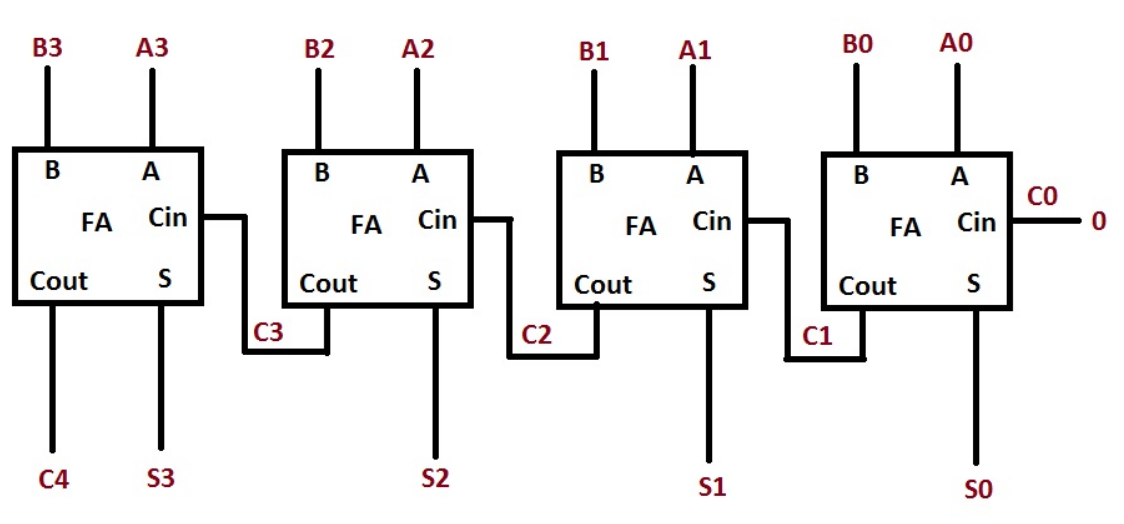
\includegraphics[width=0.7\textwidth]{rippleAdder.png}
\end{figure}

\rem{Note how the carry from each previous operation is passed onto the next, just like how one does addition manually}

\rem{Subtraction can be done much in the some way, by first applying 2's c to one of the inputs}

\newpage

\section{Synchronous Circuits}

\par{Given that logic gates are physical devices, it sometimes happens that there is a time delay between an input change and the new output. This means that it often happens that the boolean laws are not followed}

\rem{Even though the time delay for a gate is marginal, for a whole circuit the delays add up}

\defn{Gate Delay}{Time taken for a gate to respond to a change of input with the correct output}

\ex{ \begin{figure}[h]
\centering
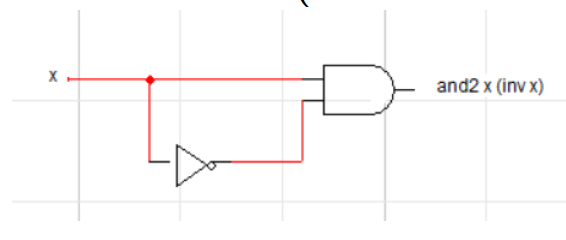
\includegraphics[width=0.5\textwidth]{gateDelay}
\end{figure}

\par{The expected output of the following circuit would be $0$, however when changing from, $1 \text{ to } 0$, the delay of the inv gate will cause both inputs of the and gate to be $1$, which in turn will erroneously output a $1$ }}

\defn{State}{!!!!GOOGLE PROPER DEFINITION}

\defn{Delay Flip Flop (dff)}{component which endows a circuit with state. It has 2 inputs (saved value, clock tick) and 1 output (state value)}

\par{Every time the \ita{dff} receives a clock signal, it updates its state value~\mymarginpar{There is only one clock signal for all flip flops, hence they are all updated simultaneously}. Since the physical components deal with analogue signals, the \ita{clock tick} can not be represented discretely. The workaround is to have the \ita{dff} treat the voltage spike as the tick}

\begin{minipage}{\linewidth}
      \centering
      \begin{minipage}{0.45\linewidth}
          \begin{figure}[H]
              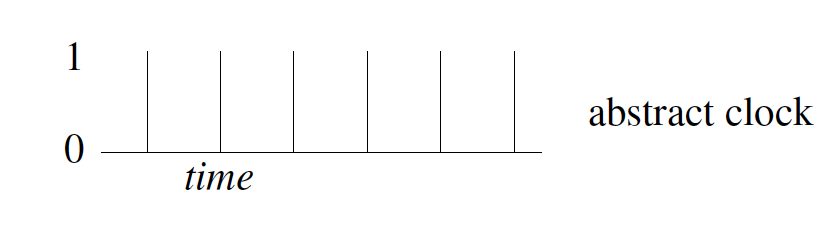
\includegraphics[width=\linewidth]{clock}
          \end{figure}
      \end{minipage}
      \hspace{0.05\linewidth}
\begin{minipage}{0.45\linewidth}
          \begin{figure}[H]
              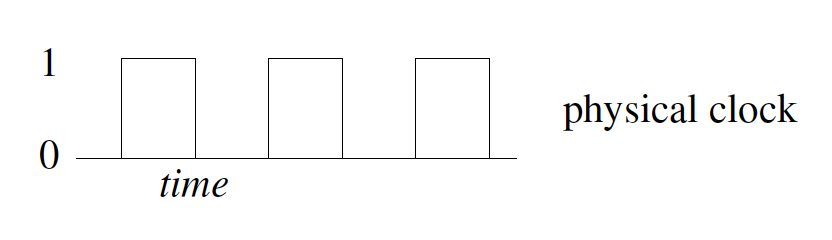
\includegraphics[width=\linewidth]{clock2}
          \end{figure}
      \end{minipage}
\end{minipage}


\defn{Synchronous Circuit}{
	\begin{enumerate}
		\item Every flip flop must be directly connected to a global clock
		\item No logical functions can be applied to the clock signal
		\item Every clock tick much reach all flip flops simultaneously
		\item Every feedback loop must pass through a flip flop
		\item The inputs to the circuit remain stable throughout clock cycles~\mymarginpar{The cycle must be long enough to allow for all signals to become valid}
	\end{enumerate}
}


\par{At every clock tick the \ita{dff} state gets updated, in order to store its state for longer we can use a register (\ita{reg1}). If the control input is 1, then the value from the \ita{dff} is loaded into the \ita{reg1} otherwise it remains the same. The conditional is implemented by an \ita{mux1}}

\defn{Register}{Allows the bit to be recorded between cycles, until a new value is loaded. It takes 2 inputs (ld =1,0 and bit) and it outputs the state bit}

\begin{figure}[h]
\centering
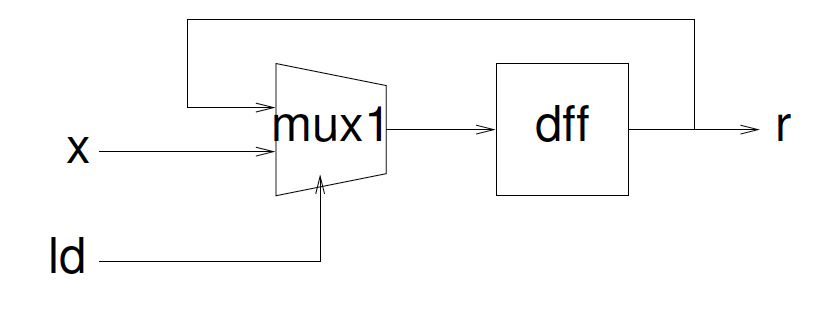
\includegraphics[width=0.7\textwidth]{reg1}
\end{figure}

$$\text{\textbf{dff\_input} $=$ mux1 ld old\_state x}$$

\par{The register can be simulated by way of a simulation table: \\}
$$
\begin{tabular}{|c|c|c|c|c|}
	Cycle & \multicolumn{2}{c}{Inputs}{} & State & Internal \\
	\hline
	& \multicolumn{2}{c}{Id}{x}  & r & dff\_input \\
	\hline
	0 & \multicolumn{2}{c}{1}{1} & ? & \textbf{1} \\
	1 & \multicolumn{2}{c}{1}{0} & \textbf{1} & \underline{0}\\
	2 & \multicolumn{2}{c}{0}{1} & \underline{0} & \textbf{0}  \\
	3 & \multicolumn{2}{c}{1}{1}  & \textbf{0} & 1 \\ 
\end{tabular}$$

\section{Register Transfer Machine}

\lecture{25}{01}{2019}



\newpage
\nocite{*}
\printbibliography


\end{document}